\section{Model}\label{sec:model}

We consider a rectangular 2D domain $\Omega\subset\mathbb{R}^2$ with boundaries 
$\partial\Omega_{1\ldots 4}\subset\partial\Omega$, shown in Fig.~\ref{fig:domain}.

\begin{figure}[!ht]
  \begin{centering}
  \includegraphics[width=0.2\columnwidth]{domain}
  \caption{\label{fig:domain} Calculation domain $\Omega\subset\mathbb{R}^2$
  	with boundaries $\partial\Omega_{1\ldots 4}\subset\partial\Omega$.}
  \end{centering}
\end{figure}

As there is no flow through the domain's boundary, Eq.~\eqref{eq:nernst-planck}
is equipped with a Neumann boundary condition 
\begin{equation}
  -D \frac{\partial C}{\partial n} - \mu F C \frac{\partial \phi} {\partial n} = 0.
  \label{eq:nernst-planck-boundary}
\end{equation}
Furthermore, we prescribe a positive constant voltage $V_{pos}$ 
on $\Omega_1$ and zero voltage on $\Omega_3$:
\begin{eqnarray}
  \phi_{\partial\Omega_1}&=&V_{pos},\\
  \phi_{\partial\Omega_3}&=&0.
  \label{eq:dirichlet}
\end{eqnarray}
On the rest of the boundary, $\phi$ has zero normal derivatives, and thus we prescribe 
a Neumann boundary condition
\begin{equation}
  \frac{\partial \phi_{\Omega_2}}{\partial n}=\frac{\partial \phi_{\Omega_4}}{\partial n}=0.
\end{equation}


\subsection{Weak form of the PNP system}

To make our results easily reproducible, in the following we present the derivation 
of weak forms of Eqs.~\eqref{eq:nernst-planck} and 
\eqref{eq:poisson}, as well as formulas for the Jacobian matrix and residual 
vector that are used in actual computations.
To simplify notation, we use dimensionless formulation of Eqs.~\eqref{eq:nernst-planck}
and~\eqref{eq:poisson}. The following new notations for the independent variables
$x$, $y$, $t$ and for the dependent variables $C$ and $\phi$ are used~\cite{bazant2004diffuse}:
\begin{equation}
  X=\frac xL,\ \ \
  Y=\frac yL,\ \ \
  \tau=\frac{tD}{\lambda_D L},\ \ \
  \varphi=\frac{\phi F}{RT},\ \ \
  c=\frac C C_0.\label{eq:dimensionless}
\end{equation}
Here $\lambda_D$ is the Debye screening length and it is expressed as follows~\cite{bazant2004diffuse}:
\begin{equation}
  \lambda_D=\sqrt{\frac{\varepsilon R T}{2 F^2 C_0}}.\label{eq:debye}
\end{equation}
After inserting variables~\eqref{eq:dimensionless} into Eq.~\eqref{eq:nernst-planck} the Nernst-Planck
equation and Poisson equation become:
\begin{eqnarray}
  \frac{DC_0}{\lambda_D L}\frac{\partial c}{\partial \tau} + \frac 1L \nabla_d\cdot
    \left(-\frac{DC_0}{L}\nabla_dc-c\frac{DC_0}{L}\nabla_d\varphi\right) &=& 0\label{eq:dim1}\\
  - \frac{\varepsilon R T}{L^2F^2C_0}\nabla_d\varphi&=&c-1\label{eq:dim2},
\end{eqnarray}
where
\begin{equation}
  \nabla_d=\left(\frac{\partial}{\partial X},\ \frac{\partial}{\partial Y}\right).
\end{equation}
After simplifying Eqs.~\eqref{eq:dim1} and~\eqref{eq:dim2} and denoting
\begin{equation}
  \epsilon=\frac{\lambda_D}{L},
\end{equation}
the dimensionless form of the PNP system of equations is
\begin{eqnarray}
  \frac{\partial c}{\partial \tau} + \epsilon \nabla_d\cdot
    \left(-\nabla_d c - c \nabla_d \varphi\right) &=&0,\label{eq:dimensionless-nernst-planck}\\
  -2\epsilon^2\nabla_d\varphi&=&c-1\label{eq:dimensionless-poisson}.
\end{eqnarray}
Boundary condition Eq.~\eqref{eq:nernst-planck-boundary} has the form
\begin{equation}
  -\frac{\partial c}{\partial n}-c\frac{\partial\varphi}{\partial n}=0.
  \label{eq:dimensionless-nernst-planck-boundary}
\end{equation}
As the second derivatives of both $c$ and $\varphi$ are present in the 
equations, the appropriate function space for them is the Sobolev space 
$V=H^1\left(\Omega\right)$ where 
$$H^1\left(\Omega\right)=\left\{v\in L^2\left(\Omega\right);\ \nabla v \in \left[L^2\left(\Omega\right)\right]^2\right\}.
$$
In order to derive the weak form of the Nernst-Planck equation Eq.~\eqref{eq:dimensionless-nernst-planck},
we first multiply it with a test function $v^c \in V$ and integrate over the domain~$\Omega$,
\begin{equation}
  \int_{\Omega}\frac{\partial C}{\partial t}v^C d\mathbf{x}
  -\int_{\Omega}D\nabla^2Cv^C d\mathbf{x}-\int_{\Omega}K\nabla C\cdot\nabla\phi v^C d\mathbf{x}
   - \int_{\Omega}KC\nabla^2\phi v^C d\mathbf{x}=0.
  \label{eq:nernst-planck-weak1}
\end{equation}
Applying the Green's first identity to the terms that contain second derivatives,
we obtain
$$
 \int_{\Omega}\frac{\partial C}{\partial t}v^C d\mathbf{x}+
  D\int_{\Omega}\nabla C\cdot\nabla v^C d\mathbf{x}-
  K\int_{\Omega}\nabla C \cdot \nabla \phi v^C d\mathbf{x}
$$
\begin{equation}
  + K\int_{\Omega}\nabla\left(Cv^C\right)\cdot \nabla \phi d\mathbf{x}
  -D\int_{\partial\Omega}\frac{\partial C}{\partial n}v^C d\mathbf{S}-
  \int_{\partial\Omega}K\frac{\partial\phi}{\partial n}Cv^C d\mathbf{S}=0.
  \label{eq:nernst-planck-weak2}
\end{equation}
Expanding the nonlinear term and using the boundary condition 
\eqref{eq:nernst-planck-boundary-2}, we have
$$
  \int_{\Omega}\frac{\partial C}{\partial t}v^C d\mathbf{x}+
  D\int_{\Omega}\nabla C \cdot \nabla v^C d\mathbf{x}-
  K\int_{\Omega}\nabla C \cdot \nabla \phi v^C d\mathbf{x}
$$
\begin{equation}
  + K\int_{\Omega}\nabla \phi \cdot \nabla C v^C d\mathbf{x}+
  K\int_{\Omega} C \left(\nabla\phi\cdot\nabla v^C\right) d\mathbf{x}=0.
  \label{eq:nernst-planck-weak3}
\end{equation}
After the second and third terms cancel out, we obtain the final weak form of 
the Nernst-Planck equation
\begin{equation}
  \int_{\Omega}\frac{\partial C}{\partial t}v^C d\mathbf{x}+
  D\int_{\Omega}\nabla C \cdot \nabla v^C d\mathbf{x}+
  K\int_{\Omega} C \left(\nabla\phi\cdot\nabla v^C\right) d\mathbf{x}=0.
  \label{eq:nernst-planck-weak-final}
\end{equation}
Analogously we derive also the weak form of the Poisson equation (\ref{eq:poisson-2}),
\begin{equation}
  -\int_{\Omega}\nabla^2\phi v^\phi d\mathbf{x}-\int_{\Omega}LCv^\phi d\mathbf{x}+
  \int_{\Omega}LC_{0}v^\phi d\mathbf{x}=0.
  \label{eq:poisson-weak1}
\end{equation}
Performing integration by parts and taking into account the boundary 
conditions for $\phi$, we obtain
\begin{equation}
  \int_{\Omega}\nabla\phi\cdot\nabla v^\phi d\mathbf{x}-\int_{\Omega}LCv^\phi d\mathbf{x}+
  \int_{\Omega}LC_{0}v^\phi d\mathbf{x}=0.
  \label{eq:poisson-weak-final}
\end{equation}


\subsection{Jacobian matrix and residual vector for the Newton's method}
To employ the Newton's method for the nonlinear system \eqref{eq:nernst-planck-weak-final},
\eqref{eq:poisson-weak-final}, formulas for the Jacobian matrix and residual vector need to
be derived. Time discretization will be performed using the second-order Crank-Nicolson 
method. The unknown solution components 
$C^{n+1}$ and $\phi^{n+1}$ at the end of the time step are expressed 
as linear combinations of finite element basis functions $v_k^{C}$ 
and $v_k^{\phi}$ with unknown coefficients,
\begin{eqnarray}
  C^{n+1} = C(Y^{n+1}) &=& \sum_{k=1}^{N^C} y_k^{C} v_k^{C}, \label{eq:cnotation}\\
  \phi^{n+1} = \phi(Y^{n+1}) &=& \sum_{k=1}^{N^{\phi}} y_k^{\phi} v_k^{\phi}\label{eq:phinotation}.
\end{eqnarray}
Here $Y^{n+1}$ is a coefficient vector of length $N^C + N^{\phi}$ comprising the unknown 
solution coefficients $y_k^{C}$ and $y_k^{\phi}$ (in this order). We will also be 
using $C^n = C(Y^n)$ and $\phi^n = \phi(Y^n)$ for the previous time step solutions.

With the notation~\eqref{eq:cnotation}, \eqref{eq:phinotation}, the time discretized 
Eq.~\eqref{eq:nernst-planck-weak-final} leads to the formula for the 
first part $F^C$ of the residual vector $F$,
\begin{eqnarray}
  F_i^C\left(Y\right) & = & \int_{\Omega} \frac{C(Y)}{\tau}v_i^C d\mathbf{x} - 
  \int_{\Omega} \frac{C^{n}}{\tau}v_i^C d\mathbf{x}\nonumber\\
  &&+\frac 12 \left[D\int_{\Omega} \nabla C(Y) \cdot \nabla v_i^C d\mathbf{x}+ 
  	D\int_{\Omega} \nabla C^{n} \cdot \nabla v_i^C d\mathbf{x}\right]\nonumber\\
  &&+ \frac 12 \left[K\int_{\Omega}C(Y) \left(\nabla \phi(Y) \cdot \nabla v_i^C\right) d\mathbf{x}+
  K\int_{\Omega}C^{n} \left(\nabla \phi^{n} \cdot \nabla v_i^C\right) d\mathbf{x}\right]\label{eq:Fc}
\end{eqnarray}
where $i = 1, 2, \ldots, N^C$.
Analogously, Eq.~\eqref{eq:poisson-weak-final} defines the second part $F^{\phi}$ 
of the residual vector $F$,
\begin{equation}
  F_i^{\phi}\left(Y\right) = \int_{\Omega} \nabla \phi(Y) \cdot \nabla v_i^{\phi} d\mathbf{x} 
  - \int_{\Omega} LC(Y)v_i^{\phi} d\mathbf{x} + \int_{\Omega} LC_0 v_i^{\phi} d\mathbf{x}
  \label{eq:Fphi}
\end{equation}
where $i = N^C + 1, N^C + 2, \ldots, N^C + N^{\phi}$. The nonlinear discrete problem 
that needs to be solved at the end of each time step thus has the form 
$F(Y) = 0$.

\newpage

\noindent
The Jacobian matrix $J(Y) = DF/DY$ has a $2\times 2$ block structure,
\begin{equation}
J(Y) = \left(
\begin{array}{cc}
  \displaystyle \frac{\partial F_i^C}{\partial y_j^C} & \displaystyle \frac{\partial F_i^C}{\partial y_j^{\phi}} \\ 
  \displaystyle \frac{\partial F_i^{\phi}}{\partial y_j^C} & \displaystyle \frac{\partial F_i^{\phi}}{\partial y_j^{\phi}}
\end{array}
\right),
\end{equation}
and its entries are obtained by calculating the partial derivatives of $F$ with
respect to the components of the coefficient vector $Y$. For this it is useful to 
realize that 
$$
\frac{\partial C(Y)}{\partial y_j^C} = v_j^C, \ \ \ 
\frac{\partial \nabla C(Y)}{\partial y_j^C} = \nabla v_j^C,\ \ \ \mbox{etc.}.
$$
We obtain
\begin{eqnarray}
  \frac{\partial F_i^C}{\partial y_j^C}(Y) &=& 
  \int_{\Omega} \frac{1}{\tau} v_j^C v_i^C d\mathbf{x} + 
  \frac 12 D\int_{\Omega} \nabla v_j^C \cdot \nabla v_i^C d\mathbf{x}
  + \frac 12 K\int_{\Omega} v_j^C \left(\nabla \phi(Y) \cdot \nabla v_i^C\right) d\mathbf{x},\label{eq:dFcdyc}\\
  \frac{\partial F_i^C}{\partial y_j^{\phi}}(Y) &=&
  \frac 12 K \int_{\Omega} C(Y) \left(\nabla v_j^{\phi} \cdot \nabla v_i^C\right) d\mathbf{x},\\
  \frac{\partial F_i^{\phi}}{\partial y_j^C}(Y) &=&
  - \int_{\Omega} L v_j^C v_i^{\phi} d\mathbf{x},\\
  \frac{\partial F_i^{\phi}}{\partial y_j^{\phi}}(Y) &=&
  \int_{\Omega} \nabla v_j^{\phi} \cdot \nabla v_i^{\phi} d\mathbf{x}\label{eq:dFphidyphi}.
\end{eqnarray}

\subsection{Newton's iteration}
At the beginning of the $(n+1)$st time step we 
set $Y^{n+1}_0 = Y^n$, where $Y^n$ is the coefficient vector  
that was calculated in the $n$th time step (or coming from the 
initial condition if $n = 0$). We set $k = 0$ and run the 
Newton's iteration 
\begin{eqnarray*}
J(Y^{n+1}_k) \delta Y^{n+1}_{k+1} &=& -F(Y^{n+1}_k), \\ 
Y^{n+1}_{k+1} &=& Y^{n+1}_k + \delta Y^{n+1}_{k+1}, \\
k &:=& k+1
\end{eqnarray*}
over $k$ until it converges. Then we set $Y^{n+1} := Y^{n+1}_{k}$. 
We use a combined stopping criterion 
that makes sure that both the norm of the residual vector $\Vert F(Y^{n+1})\Vert$ 
as well as the norm of the increment $\Vert \delta Y^{n+1}\Vert$ are sufficiently 
small.

\section{Adaptive $hp$-FEM and the Open-Source Library Hermes}
\label{sec:hermes}

In traditional low-order FEM (based on piecewise-linear or piecewise quadratic elements), 
refining an element is not algorithmically complicated,
and so the most difficult part is to find out what elements should be refined. 
To do this, various techniques ranging from rigorous guaranteed a-posteriori 
error estimates to heuristic criteria such as residual error indicators or
error indicators based on steep gradients are employed. 

However, none of these approaches is suitable for
multiphysics coupled problems or higher-order finite element methods: 
Rigorous guaranteed error estimates only exist for very simple problems 
(such as linear elliptic PDE) and only for low-order finite elements.
Heuristic techniques are usually somehow doable for all problems, but 
they fail in more complicated situations. Moreover, they lack a 
transparent relation to the true approximation error and thus they may
give wrong results.

Automatic adaptivity in higher-order finite element methods (\emph{hp}-FEM) 
is much different from adaptivity in low-order FEM. Firstly, analytical
error estimates capable of guiding adaptive $hp$-FEM do not exist even for 
the simplest linear elliptic equations, not speaking about nonlinear multiphysics 
coupled systems. Secondly,
a higher-order element can be refined in many different ways, as illustrated 
in Fig.~\ref{fig:refinements}.
\begin{figure}[!ht]
  \begin{centering}
  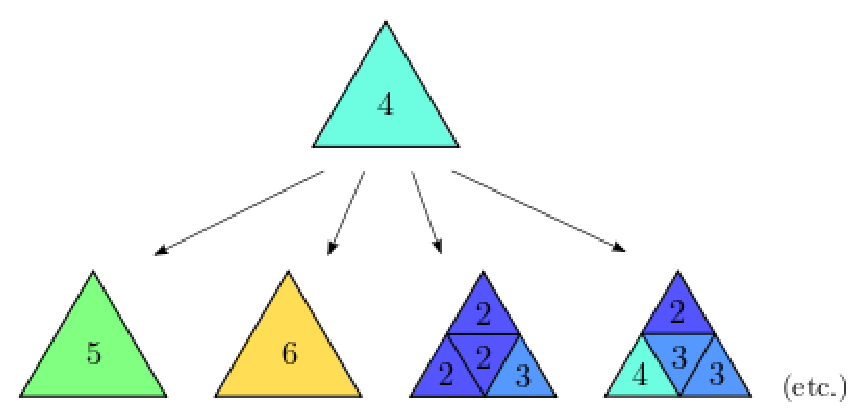
\includegraphics[width=0.5\columnwidth]{refinements}
  \caption{\label{fig:refinements} Many possible refinement candidates for a fourth-order
  element.}
  \end{centering}
%\vspace{-0.5cm}
\end{figure}

%\newpage
The number of possible element refinements is implementation dependent. 
In general it is very low in \emph{h}-adaptivity and \emph{p}-adaptivity, 
and much higher in \emph{hp}-adaptivity. Moreover, this number grows very 
fast when anisotropic refinements are enabled.

\subsection{The Hermes Library}

Hermes\footnote{http://hpfem.org/hermes} is a free and open-source C++ library 
that implements higher-order finite elements approximations and adaptive $hp$-FEM.
It supports 8 different adaptivity modes -- three isotropic and five anisotropic. 
The isotropic refinements are
\emph{h}-isotropic (H\_ISO), \emph{p}-isotropic (P\_ISO), \emph{hp}-isotropic (HP\_ISO).
Anisotropic refinement modes are
\emph{h}-anisotropic (H\_ANISO),
\emph{hp}-anisotropic-\emph{h} (HP\_ANISO\_H), \emph{p}-anisotropic (P\_ANISO),
\emph{hp}-anisotropic-p (HP\_ANISO\_P), and \emph{hp}-anisotropic (HP\_ANISO).
The eight adaptivity modes are summarized in Fig.~\ref{fig:candlist}. It must
be noted that in case of HP\_ANISO\_H, only element size is adapted anisotropically
whereas polynomial degree is adapted isotropically. The opposite holds true
for HP\_ANISO\_P.

\begin{figure}[!ht]
  \begin{centering}
  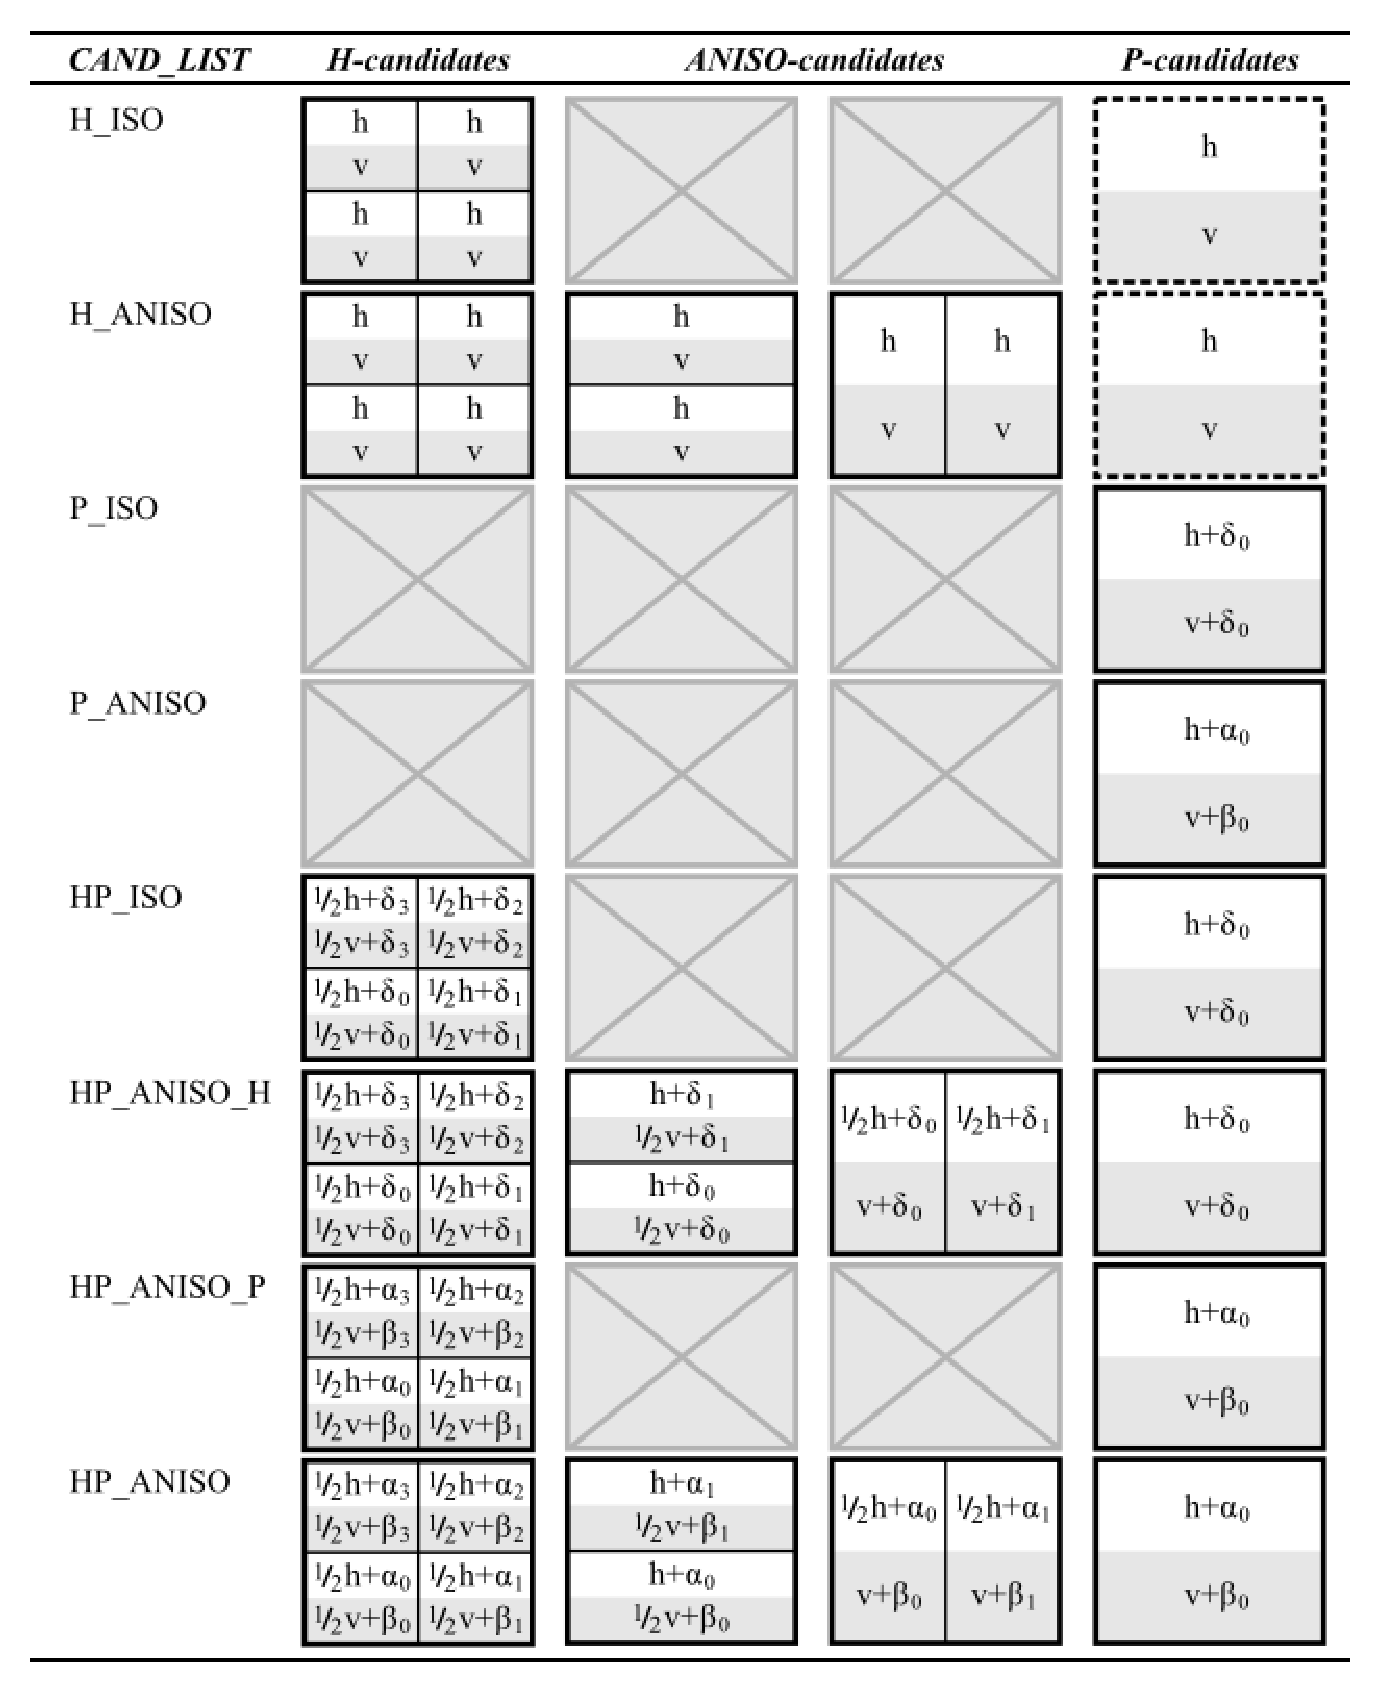
\includegraphics[width=0.8\columnwidth]{cand_list_quads}
  \caption{\label{fig:candlist} Refinement candidates for every
  refinement mode for quad type elements.}
  \end{centering}
\end{figure}
Note that triangular elements do not support anisotropic refinements.
Due to the large number of refinement options, classical error estimators 
that provide a constant error estimate per element, cannot be used to 
guide automatic \emph{hp}-adaptivity. 
For this, one needs to know the shape of the approximation error.
Hermes uses a pair of approximations with different orders of accuracy 
to obtain this information: coarse mesh solution and fine mesh solution~\cite{solin2010pde}. 
The initial coarse mesh is read from the mesh file, and the initial 
fine mesh is created through its global refinement both in \emph{h}
and \emph{p}. The fine mesh solution is the approximation of 
interest both during the adaptive process and at the end of computation. 
Global orthogonal projection of the fine mesh solution on the coarse mesh 
is used to extract the low-order part from the reference solution.
The adaptivity algorithm is guided by the difference between the 
reference solution and its low-order part.
Note that this approach to automatic adaptivity is PDE-independent
and thus naturally applicable to a large variety of multiphysics 
coupled problems.

\subsection{Multimesh $hp$-FEM}
In multiphysics PDE systems such as Poisson-Nernst-Planck it can 
happen that one physical field is very smooth where others are not,
as we illustrated in Fig.~\ref{fig:comsol-conc-volt}. 
If all the fields are approximated on the same mesh, then 
unnecessary refinements will be present in smooth areas
where they are not necessary. This can be very wasteful.

Hermes implements a novel adaptive multimesh $hp$-FEM~\cite{solin2010monolithic,
solin2010adaptive,dubcova2010space}
that makes it possible to approximate different fields on individual meshes,
without breaking the monolithic structure of the coupling mechanism.
For practical reasons, the meshes in the system are not allowed to be 
completely independent -- they have a common coarse mesh that we call {\em 
master mesh}. The master mesh is 
there for algorithmic purposes only and it may not even be used for 
discretization purposes. Every mesh in the system is obtained from 
the master mesh via an arbitrary sequence of elementary refinements. 
Assembling is done on a {\em union mesh}, a geometrical union of 
all meshes in the system (imagine printing all meshes on transparencies and 
positioning them on top of each other). 

The union mesh is not constructed physically in the computer 
memory -- it merely serves as a hint to correctly transform the 
integration points while integrating over sub-elements of elements 
in the existing meshes. 
As a result, the multimesh discretization of the PDE system is 
monolithic in the sense that no physics is lost --- all integrals 
in the discrete weak formulations are evaluated exactly up to 
the error in the numerical quadrature. The exact preservation of 
the coupling structure of multiphysics coupled problems makes 
the multimesh $hp$-FEM very different from various interpolation 
and projection based methods that suffer from errors made
while transferring data between different meshes in the system. 


